\documentclass[DIV=14,titlepage=false]{scrreprt}
\usepackage{parskip}
%%%%%%%%%%%%%%%%%%%%%%%%%%%%%%%%%%%%%%%%%%%%%%%%%%%%%%%%%%%%%%%%%%%%%%%%%%%%%%%
%                                Basic Packages                               %
%%%%%%%%%%%%%%%%%%%%%%%%%%%%%%%%%%%%%%%%%%%%%%%%%%%%%%%%%%%%%%%%%%%%%%%%%%%%%%%
% Gives us multiple colors.
\usepackage[usenames,dvipsnames,pdftex]{xcolor}
% Lets us style link colors.
\usepackage{hyperref}
% Lets us import images and graphics.
\usepackage{graphicx}
% Lets us use figures in floating environments.
\usepackage{float}
% Lets us create multiple columns.
\usepackage{multicol}
% Gives us better math syntax.
\usepackage{amsmath,amsfonts,mathtools,amsthm,amssymb}
% Lets us strikethrough text.
\usepackage{cancel}
% Lets us edit the caption of a figure.
\usepackage{caption}
% Lets us import pdf directly in our tex code.
\usepackage{pdfpages}
% Lets us do algorithm stuff.
\usepackage[ruled,vlined,linesnumbered]{algorithm2e}
% Gets rid of some errors.
\usepackage{scrhack}
\def\class{article}
\usepackage{geometry}
\geometry{margin=0.9in}
%%%%%%%%%%%%%%%%%%%%%%%%%%%%%%%%%%%%%%%%%%%%%%%%%%%%%%%%%%%%%%%%%%%%%%%%%%%%%%%
%                                Basic Settings                               %
%%%%%%%%%%%%%%%%%%%%%%%%%%%%%%%%%%%%%%%%%%%%%%%%%%%%%%%%%%%%%%%%%%%%%%%%%%%%%%%

%%%%%%%%%%%%%
%  Symbols  %
%%%%%%%%%%%%%

\let\implies\Rightarrow
\let\impliedby\Leftarrow
\let\iff\Leftrightarrow
\let\epsilon\varepsilon

%%%%%%%%%%%%
%  Tables  %
%%%%%%%%%%%%

\setlength{\tabcolsep}{5pt}
\renewcommand\arraystretch{1.5}

%%%%%%%%%%%%%%%%%%%%%%%
%  Center Title Page  %
%%%%%%%%%%%%%%%%%%%%%%%

\usepackage{titling}
\renewcommand\maketitlehooka{\null\mbox{}\vfill}
\renewcommand\maketitlehookd{\vfill\null}

%%%%%%%%%%%%%%%%%%%%%%%%%%%%%%%%%%%%%%%%%%%%%%%%%%%%%%%
%  Create a grey background in the middle of the PDF  %
%%%%%%%%%%%%%%%%%%%%%%%%%%%%%%%%%%%%%%%%%%%%%%%%%%%%%%%

\usepackage{eso-pic}
\newcommand\definegraybackground{
  \definecolor{reallylightgray}{HTML}{FAFAFA}
  \AddToShipoutPicture{
    \ifthenelse{\isodd{\thepage}}{
      \AtPageLowerLeft{
        \put(\LenToUnit{\dimexpr\paperwidth-222pt},0){
          \color{reallylightgray}\rule{222pt}{297mm}
        }
      }
    }
    {
      \AtPageLowerLeft{
        \color{reallylightgray}\rule{222pt}{297mm}
      }
    }
  }
}

%%%%%%%%%%%%%%%%%%%%%%%%
%  Modify Links Color  %
%%%%%%%%%%%%%%%%%%%%%%%%

\hypersetup{
  % Enable highlighting links.
  colorlinks,
  % Change the color of links to blue.
  linkcolor={black},
  % Change the color of citations to black.
  citecolor={black},
  % Change the color of url's to blue with some black.
  urlcolor=blue
}

%%%%%%%%%%%%%%%%%%
% Fix WrapFigure %
%%%%%%%%%%%%%%%%%%

\newcommand{\wrapfill}{\par\ifnum\value{WF@wrappedlines}>0
    \parskip=0pt
    \addtocounter{WF@wrappedlines}{-1}%
    \null\vspace{\arabic{WF@wrappedlines}\baselineskip}%
    \WFclear
\fi}

%%%%%%%%%%%%%%%%%
% Multi Columns %
%%%%%%%%%%%%%%%%%

\let\multicolmulticols\multicols
\let\endmulticolmulticols\endmulticols

\RenewDocumentEnvironment{multicols}{mO{}}
{%
  \ifnum#1=1
    #2%
  \else % More than 1 column
    \multicolmulticols{#1}[#2]
  \fi
}
{%
  \ifnum#1=1
\else % More than 1 column
  \endmulticolmulticols
\fi
}

\newlength{\thickarrayrulewidth}
\setlength{\thickarrayrulewidth}{5\arrayrulewidth}

%%%%%%%%%%%%%%%%%%%%
%  Import Figures  %
%%%%%%%%%%%%%%%%%%%%

\usepackage{import}
\pdfminorversion=7

% EXAMPLE:
% 1. \incfig{limit-graph}
% 2. \incfig[0.4]{limit-graph}
% Parameters:
% 1. The figure name. It should be located in figures/NAME.tex_pdf.
% 2. (Optional) The width of the figure. Example: 0.5, 0.35.
\newcommand\incfig[2][1]{%
  \def\svgwidth{#1\columnwidth}
  \import{./figures/}{#2.pdf_tex}
}

\begingroup\expandafter\expandafter\expandafter\endgroup
\expandafter\ifx\csname pdfsuppresswarningpagegroup\endcsname\relax
\else
  \pdfsuppresswarningpagegroup=1\relax
\fi

%%%%%%%%%%%%%
%  Correct  %
%%%%%%%%%%%%%

% EXAMPLE:
% 1. \correct{INCORRECT}{CORRECT}
% Parameters:
% 1. The incorrect statement.
% 2. The correct statement.
\definecolor{correct}{HTML}{009900}
\newcommand\correct[2]{{\color{red}{#1 }}\ensuremath{\to}{\color{correct}{ #2}}}



\newcommand{\R}{\mathbb{R}}
\newcommand{\Z}{\mathbb{Z}}
\newcommand{\E}{\mathbb{E}}
\newcommand{\B}{\ensuremath{\mathcal{B}}}
\newcommand{\X}{\ensuremath{\mathcal{X}}}
\newcommand{\Y}{\ensuremath{\mathcal{Y}}}
\newcommand{\mA}{\ensuremath{\mathbf{A}}}
\newcommand{\mB}{\ensuremath{\mathbf{B}}}
\newcommand{\mC}{\ensuremath{\mathbf{C}}}
\newcommand{\mD}{\ensuremath{\mathbf{D}}}
\newcommand{\mX}{\ensuremath{\mathbf{X}}}
\newcommand{\mY}{\ensuremath{\mathbf{Y}}}
\newcommand{\mx}{\ensuremath{\mathbf{x}}}
\newcommand{\my}{\ensuremath{\mathbf{y}}}
\newcommand{\mI}{\ensuremath{\mathbf{I}}}
\newcommand{\mi}{\ensuremath{\mathbf{\iota}}}
\newcommand{\mmu}{\ensuremath{\mathbf{\mu}}}
\newcommand{\mc}{\ensuremath{\mathbf{c}}}
\newcommand{\mSigma}{\ensuremath{\mathbf{\Sigma}}}
\newcommand{\mzero}{\ensuremath{\mathbf{0}}}
\newcommand{\independent}{\perp\!\!\!\!\perp} 
\setlength{\parindent}{0pt}
%%%%%%%%%%%%%%%%%%%%%%%%%%%%%%%%%%%%%%%%%%%%%%%%%%%%%%%%%%%%%%%%%%%%%%%%%%%%%%%
%                                 Environments                                %
%%%%%%%%%%%%%%%%%%%%%%%%%%%%%%%%%%%%%%%%%%%%%%%%%%%%%%%%%%%%%%%%%%%%%%%%%%%%%%%

\usepackage{varwidth}
\usepackage{thmtools}
\usepackage[most,many,breakable]{tcolorbox}

\tcbuselibrary{theorems,skins,hooks}
\usetikzlibrary{arrows,calc,shadows.blur}

%%%%%%%%%%%%%%%%%%%
%  Define Colors  %
%%%%%%%%%%%%%%%%%%%

\definecolor{myblue}{RGB}{45, 111, 177}
\definecolor{mygreen}{RGB}{56, 140, 70}
\definecolor{myred}{RGB}{199, 68, 64}
\definecolor{mypurple}{RGB}{197, 92, 212}

\definecolor{definition}{HTML}{228b22}
\definecolor{theorem}{HTML}{00007B}
\definecolor{example}{HTML}{2A7F7F}
\definecolor{definition}{HTML}{228b22}
\definecolor{prop}{HTML}{191971}
\definecolor{lemma}{HTML}{983b0f}
\definecolor{exercise}{HTML}{88D6D1}

\colorlet{definition}{mygreen!85!black}
\colorlet{claim}{mygreen!85!black}
\colorlet{corollary}{mypurple!85!black}
\colorlet{proof}{theorem}

%%%%%%%%%%%%%%%%%%%%%%
%  Helpful Commands  %
%%%%%%%%%%%%%%%%%%%%%%

% EXAMPLE:
% 1. \createnewtheoremstyle{thmdefinitionbox}{}{}
% 2. \createnewtheoremstyle{thmtheorembox}{}{}
% 3. \createnewtheoremstyle{thmproofbox}{qed=\qedsymbol}{
%       rightline=false, topline=false, bottomline=false
%    }
% Parameters:
% 1. Theorem name.
% 2. Any extra parameters to pass directly to declaretheoremstyle.
% 3. Any extra parameters to pass directly to mdframed.
\newcommand\createnewtheoremstyle[3]{
  \declaretheoremstyle[
  headfont=\bfseries\sffamily, bodyfont=\normalfont, #2,
  mdframed={
    #3,
  },
  ]{#1}
}

% EXAMPLE:
% 1. \createnewcoloredtheoremstyle{thmdefinitionbox}{definition}{}{}
% 2. \createnewcoloredtheoremstyle{thmexamplebox}{example}{}{
%       rightline=true, leftline=true, topline=true, bottomline=true
%     }
% 3. \createnewcoloredtheoremstyle{thmproofbox}{proof}{qed=\qedsymbol}{backgroundcolor=white}
% Parameters:
% 1. Theorem name.
% 2. Color of theorem.
% 3. Any extra parameters to pass directly to declaretheoremstyle.
% 4. Any extra parameters to pass directly to mdframed.
\newcommand\createnewcoloredtheoremstyle[4]{
  \declaretheoremstyle[
  headfont=\bfseries\sffamily\color{#2}, bodyfont=\normalfont, #3,
  mdframed={
    linewidth=2pt,
    rightline=false, leftline=true, topline=false, bottomline=false,
    linecolor=#2, backgroundcolor=#2!5, #4,
  },
  ]{#1}
}

%%%%%%%%%%%%%%%%%%%%%%%%%%%%%%%%%%%
%  Create the Environment Styles  %
%%%%%%%%%%%%%%%%%%%%%%%%%%%%%%%%%%%

\makeatletter
\@ifclasswith\class{nocolor}{
  % Environments without color.

  \createnewtheoremstyle{thmdefinitionbox}{}{}
  \createnewtheoremstyle{thmtheorembox}{}{}
  \createnewtheoremstyle{thmexamplebox}{}{}
  \createnewtheoremstyle{thmclaimbox}{}{}
  \createnewtheoremstyle{thmcorollarybox}{}{}
  \createnewtheoremstyle{thmpropbox}{}{}
  \createnewtheoremstyle{thmlemmabox}{}{}
  \createnewtheoremstyle{thmexercisebox}{}{}
  \createnewtheoremstyle{thmdefinitionbox}{}{}
  \createnewtheoremstyle{thmquestionbox}{}{}
  \createnewtheoremstyle{thmsolutionbox}{}{}

  \createnewtheoremstyle{thmproofbox}{qed=\qedsymbol}{}
  \createnewtheoremstyle{thmexplanationbox}{}{}
}{
  % Environments with color.

  \createnewcoloredtheoremstyle{thmdefinitionbox}{definition}{}{}
  \createnewcoloredtheoremstyle{thmtheorembox}{theorem}{}{}
  \createnewcoloredtheoremstyle{thmexamplebox}{example}{}{
    rightline=true, leftline=true, topline=true, bottomline=true
  }
  \createnewcoloredtheoremstyle{thmclaimbox}{claim}{}{}
  \createnewcoloredtheoremstyle{thmcorollarybox}{corollary}{}{}
  \createnewcoloredtheoremstyle{thmpropbox}{prop}{}{}
  \createnewcoloredtheoremstyle{thmlemmabox}{lemma}{}{}
  \createnewcoloredtheoremstyle{thmexercisebox}{exercise}{}{}

  \createnewcoloredtheoremstyle{thmproofbox}{proof}{qed=\qedsymbol}{backgroundcolor=white}
  \createnewcoloredtheoremstyle{thmexplanationbox}{example}{qed=\qedsymbol}{backgroundcolor=white}
}
\makeatother

%%%%%%%%%%%%%%%%%%%%%%%%%%%%%
%  Create the Environments  %
%%%%%%%%%%%%%%%%%%%%%%%%%%%%%

\declaretheorem[numberwithin=section, style=thmtheorembox,     name=Theorem]{theorem}
\declaretheorem[numbered=no,          style=thmexamplebox,     name=Example]{example}
\declaretheorem[numberwithin=section, style=thmclaimbox,       name=Claim]{claim}
\declaretheorem[numberwithin=section, style=thmcorollarybox,   name=Corollary]{corollary}
\declaretheorem[numberwithin=section, style=thmpropbox,        name=Proposition]{prop}
\declaretheorem[numberwithin=section, style=thmlemmabox,       name=Lemma]{lemma}
\declaretheorem[numberwithin=section, style=thmexercisebox,    name=Exercise]{exercise}
\declaretheorem[numbered=no,          style=thmproofbox,       name=Proof]{replacementproof}
\declaretheorem[numbered=no,          style=thmexplanationbox, name=Proof]{expl}

\makeatletter
\@ifclasswith\class{nocolor}{
  % Environments without color.

  \newtheorem*{note}{Note}

  \declaretheorem[numberwithin=section, style=thmdefinitionbox, name=Definition]{definition}
  \declaretheorem[numberwithin=section, style=thmquestionbox,   name=Question]{question}
  \declaretheorem[numberwithin=section, style=thmsolutionbox,   name=Solution]{solution}
}{
  % Environments with color.

  \newtcbtheorem[number within=section]{Definition}{Definition}{
    enhanced,
    before skip=2mm,
    after skip=2mm,
    colback=red!5,
    colframe=red!80!black,
    colbacktitle=red!75!black,
    boxrule=0.5mm,
    attach boxed title to top left={
      xshift=1cm,
      yshift*=1mm-\tcboxedtitleheight
    },
    varwidth boxed title*=-3cm,
    boxed title style={
      interior engine=empty,
      frame code={
        \path[fill=tcbcolback]
        ([yshift=-1mm,xshift=-1mm]frame.north west)
        arc[start angle=0,end angle=180,radius=1mm]
        ([yshift=-1mm,xshift=1mm]frame.north east)
        arc[start angle=180,end angle=0,radius=1mm];
        \path[left color=tcbcolback!60!black,right color=tcbcolback!60!black,
        middle color=tcbcolback!80!black]
        ([xshift=-2mm]frame.north west) -- ([xshift=2mm]frame.north east)
        [rounded corners=1mm]-- ([xshift=1mm,yshift=-1mm]frame.north east)
        -- (frame.south east) -- (frame.south west)
        -- ([xshift=-1mm,yshift=-1mm]frame.north west)
        [sharp corners]-- cycle;
      },
    },
    fonttitle=\bfseries,
    title={#2},
    #1
  }{def}

  \NewDocumentEnvironment{definition}{O{}O{}}
    {\begin{Definition}{#1}{#2}}{\end{Definition}}

  \newtcolorbox{note}[1][]{%
    enhanced jigsaw,
    colback=gray!20!white,%
    colframe=gray!80!black,
    size=small,
    boxrule=1pt,
    title=\textbf{Note:-},
    halign title=flush center,
    coltitle=black,
    breakable,
    drop shadow=black!50!white,
    attach boxed title to top left={xshift=1cm,yshift=-\tcboxedtitleheight/2,yshifttext=-\tcboxedtitleheight/2},
    minipage boxed title=1.5cm,
    boxed title style={%
      colback=white,
      size=fbox,
      boxrule=1pt,
      boxsep=2pt,
      underlay={%
        \coordinate (dotA) at ($(interior.west) + (-0.5pt,0)$);
        \coordinate (dotB) at ($(interior.east) + (0.5pt,0)$);
        \begin{scope}
          \clip (interior.north west) rectangle ([xshift=3ex]interior.east);
          \filldraw [white, blur shadow={shadow opacity=60, shadow yshift=-.75ex}, rounded corners=2pt] (interior.north west) rectangle (interior.south east);
        \end{scope}
        \begin{scope}[gray!80!black]
          \fill (dotA) circle (2pt);
          \fill (dotB) circle (2pt);
        \end{scope}
      },
    },
    #1,
  }

  \newtcbtheorem{Question}{Question}{enhanced,
    breakable,
    colback=white,
    colframe=myblue!80!black,
    attach boxed title to top left={yshift*=-\tcboxedtitleheight},
    fonttitle=\bfseries,
    title=\textbf{Question:-},
    boxed title size=title,
    boxed title style={%
      sharp corners,
      rounded corners=northwest,
      colback=tcbcolframe,
      boxrule=0pt,
    },
    underlay boxed title={%
      \path[fill=tcbcolframe] (title.south west)--(title.south east)
      to[out=0, in=180] ([xshift=5mm]title.east)--
      (title.center-|frame.east)
      [rounded corners=\kvtcb@arc] |-
      (frame.north) -| cycle;
    },
    #1
  }{def}

  \NewDocumentEnvironment{question}{O{}O{}}
  {\begin{Question}{#1}{#2}}{\end{Question}}

  \newtcolorbox{Solution}{enhanced,
    breakable,
    colback=white,
    colframe=mygreen!80!black,
    attach boxed title to top left={yshift*=-\tcboxedtitleheight},
    title=\textbf{Solution:-},
    boxed title size=title,
    boxed title style={%
      sharp corners,
      rounded corners=northwest,
      colback=tcbcolframe,
      boxrule=0pt,
    },
    underlay boxed title={%
      \path[fill=tcbcolframe] (title.south west)--(title.south east)
      to[out=0, in=180] ([xshift=5mm]title.east)--
      (title.center-|frame.east)
      [rounded corners=\kvtcb@arc] |-
      (frame.north) -| cycle;
    },
  }

  \NewDocumentEnvironment{solution}{O{}O{}}
  {\vspace{-10pt}\begin{Solution}{#1}{#2}}{\end{Solution}}
}
\makeatother

%%%%%%%%%%%%%%%%%%%%%%%%%%%%
%  Edit Proof Environment  %
%%%%%%%%%%%%%%%%%%%%%%%%%%%%

\renewenvironment{proof}[1][\proofname]{\vspace{-10pt}\begin{replacementproof}}{\end{replacementproof}}
\newenvironment{explanation}[1][\proofname]{\vspace{-10pt}\begin{expl}}{\end{expl}}

\theoremstyle{definition}

\newtheorem*{notation}{Notation}
\newtheorem*{previouslyseen}{As previously seen}
\newtheorem*{problem}{Problem}
\newtheorem*{observe}{Observe}
\newtheorem*{property}{Property}
\newtheorem*{intuition}{Intuition}



\title{%
R300 Econometrics}
\author{Metrics Enjoyers}
\date{Michaelmas Term, 2023-2024}

\setuptoc{toc}{leveldown}
\setcounter{chapter}{6}

\begin{document}

\chapter{Multicollinearity. Ridge and LASSO. Model Selection for Prediction. Mallow's \(C_P\) Criterion}

\subsection{Perfect Multicollinearity}

\begin{definition}[Perfect Multicollinearity]
    This defines the case where rank \((X) \neq k\) and \underline{GM1 is violated}
    \\ \\
    \(\implies \exists\) an exact linear dependence between the columns of X so that
    \[X\alpha=0 \quad \text{for some} \hspace{1mm} \alpha \neq 0\] 
\end{definition}

\vspace{5mm}

\begin{corollary}
    Models \[Y=X\beta+\epsilon \quad \text{and} \quad Y=X\tilde{\beta}+\epsilon\]
    where \(\tilde{\beta}=\beta+\lambda\alpha\) for any \(\lambda\) are equivalent. Thus \(\beta\) is \underline{not identified} as we cannot distinguish between the two.
\end{corollary}

\begin{corollary} In the OLS case, 
    rank \((X) \neq k\): \\ \\ \(\implies\) non invertability of \(X'X\) \\ \(\implies\) infinite number of solutions to the OLS problem. \(min_{b}||Y-Xb||^2\). Thus OLS estimator is not well defined.
\end{corollary}

\vspace{5mm}
\begin{example}
    Dummy Variable Trap: \\ \\
    Consider the model \(Y=\beta_0X_0+\beta_1X_1+\beta_2X_2+\epsilon\), where \(X_0\) is a constant vector \(=\vec{1}\) and \(X_1, X_2\) are dummies such that \(X_2=1-X_1\). \\ \\
    \(\implies\) \(X_2\) is a linear combination of \(X_1\) and \(X_0\) and thus model is not identified. Specifically, \(X\alpha=0, \text{for} \, \alpha = (1, -1, -1)'\) \\ \\
    \(\implies\) \(X'X\) is not invertible. \\ \\
    \(\implies\) OLS estimator is not well defined.
\end{example}

We also can have perfect multicollinearity with small sample sizes s.t. \(n<k\). Thus rank \((X) \leq n < k\).

\subsection{Imperfect Multicollinearity}
Often there will exist a linear combination of X that is almost but not exactly 0

\begin{definition} Imperfect multicollinearity
\[rank(X)=k, \quad X\alpha \approx 0 \quad \text{for some} \hspace{1mm} \alpha \neq 0\]
But this is not a unit invariant quantity, instead we can look at the relative size of the eigenvalues of \(X'X\).
\[\frac{\lambda_{max}}{\lambda_{min}}\]

\end{definition}

\vspace{5mm}

\begin{corollary}
    Multicollinearity will result in a large norm of the variance-covariance matrix of the OLS estimator \(\sigma^2(X'X)^{-1}\) and thus a very large trace.
    Trace of the variance of OLS estimator yields:
    \[tr(\sigma^2(X'X)^{-1})=E(||\hat{\beta}-\beta||^2|X)\]
    Thus large multicollinearity will mean a large expected squared distance between true and estimated value of parameters.
\end{corollary}

\begin{note}
    Norm here is defined as \(\operatorname*{max}_{\substack{x\neq0}}\frac{||Ax||}{||x||}\), \href{https://math.mit.edu/~gs/linearalgebra/ila6/ila5conditionnumbers.pdf}{more details}
\\ \\
Also:
    \[\frac{\lambda_{max}}{\lambda_{min}}\] represents the condition number \(C = ||A|| \, ||A^{-1}||\) of matrix \(X'X\) (if this matrix is positive definite and (given) symmetric)\footnote{Proof in Appendix}. 
    \underline{Intution behind condition number:}
    For a set of simulateneous equations \(Ax=b\) the condition number of \(A\) sets a bound of the sensitivity of the relative (i.e. invariant to units) solution error (in \(x\)) induced by errors in the problem vector (\(b\)). \(\frac{||\Delta x||}{||x||} \leq C \frac{||\Delta b||}{||b||}\)\footnote{Proof in Appendix}. Thus if \(C\) is large, then the solution can be very sensitive to small changes in the problem. (Worst case when \(b\) points in the smallest eigenvector direction of \(A\) and \(\Delta b\) points in the largest eigenvector direction of \(A\).) \\
    \\
    Applying this to \(X'X\), we can see that if the condition number is large, then the "solution error" in \(\beta\) can be very sensitive to small changes in the problem, i.e. small changes in \(X'Y\), i.e. \(\epsilon\). 
    Here, \(Ax=b \equiv X'X\beta=X'Y\). This shows why it is a good condition to represent the large variance of the OLS estimator in the presence of multicollinearity.
\end{note}
\newpage
\section{Ridge Regression}

By G-M the resulting large MSE is still best among any other conditionally unbiased estimator. Thus, solutions recommend minimising expected MSE via introducing bias and reducing variance.

\begin{definition}Ridge Regression Estimator: \\

    This solves the OLS problem but where size of \(||\beta||^2=\beta'\beta\) is penalised by \(\lambda\).
    \[\operatorname*{min}_{\beta}\left(||Y-X\beta||^2+\lambda||\beta||^2\right) \text{for some} \, \lambda > 0\]

    We can show this results in the estimate (for \(k< n\)):
    \[\hat{\beta}_{r}=(X'X+\lambda I)^{-1}X'Y\]

    Note: \[E(\hat{\beta}_{r}|X)=(X'X+\lambda I)^{-1}X'X\beta\] and thus \(\hat{\beta}_{r}\) is biased. When \(\lambda\) rises the bias increases and the variance decreases, illustrating the exploitable bias-variance tradeoff.
    \[Var(\hat{\beta}_{r}|X)=\sigma^2(X'X+\lambda I)^{-1}X'X(X'X+\lambda I)^{-1}\]
    We can see this explicitly by looking at the condition number of \(X'X+\lambda I\):\footnote[3]{Proof in Appendix}
    \[= \frac{\lambda_{max}+\lambda}{\lambda_{min}+\lambda}<\frac{\lambda_{max}}{\lambda_{min}}\]
    As \((X'X+\lambda I)\hat{\beta}_{r}=X'Y\), we can see that the relative solution error in \(\hat{\beta}_{r}\) is bounded by:
    \[\frac{||\Delta \hat{\beta}_{r}||}{||\hat{\beta}_{r}||} \leq \frac{\lambda_{max}+\lambda}{\lambda_{min}+\lambda}\frac{||\Delta X'Y||}{||X'Y||}\]
    Thus, as \(\lambda\) rises, the solution error in \(\hat{\beta}_{r}\) becomes less sensitive to changes in \(X'Y\), i.e. \(\epsilon\). This is the bias-variance tradeoff.
\end{definition}

\vspace{5mm}
\begin{proof}
     \[\equiv \operatorname*{min}_b (Y'Y - b'X'Y - Y'Xb + b'X'Xb + \lambda b'b)\]
     \[FOC: -X'Y-X'Y+2X'Xb+2\lambda b=0\]
     \[2(X'X+\lambda I)b=2X'Y\]
     \[b=(X'X+\lambda I)^{-1}X'Y=\hat{\beta}_r\]
\end{proof}

\subsection{Cross-Validation}
The parameter \(\lambda\) is usually chosen by CV:

Overall idea is to minimise expected squared prediction error \(E(y-x'\hat{\beta}_r)^2\), where \((y,x)\) is a new observation from the joint distribution of the dependent and explanatory variables.
As we do not have such a new observation we approximate it via the leave one out CV method:

\begin{enumerate}
    \item Drop the i-th observation \((y_i, x_i)\) from the sample
    \item Estimate \(\hat{\beta}_{r(-i)}\) on the remaining \(n-1\) observations
    \item Estimate \(E(y-x'\hat{\beta}_{-i,r})^2\) via taking the average of the squared prediction errors on the dropped observation \((y_i, x_i)\) via \(\frac{1}{n}\sum_{i=1}^{n}(y_i-x_i'\hat{\beta}_{-i,r})^2\)
    \item Choose \(\lambda\) that minimises the above estimate.
\end{enumerate}

\vspace{5mm}

\begin{example}
    \textbf{Ridge in an Overidentified Model}: \(k>n\) \\ \\
    Clearly here the classical OLS estimator would not be defined, since \(X'X\) is not invertible. Its rank is bounded by \(n\) but dimensions are \(k\times k\). Thus we need to introduce some bias to make the problem well defined.
    We note that, assuming (\(X\) is of rank \(n\)), the column space of \(X\) will span \(\mathbb{R}^n\). Thus we can find exact vectors \(b\) such that \(Xb=Y\), where multiplicity due to the fact \(k>n\). We select among these by minimising the L2 norm:
    \[\operatorname*{min}_b ||b||^2 \quad \text{subject to} \quad Xb=Y\]
    \[\mathbb{L}=b'b+\lambda'(Y-Xb)\]
    \[\text{FOC}: \begin{cases} b: 2b-X'\lambda=0 \\ \lambda: (Y-Xb)=0\end{cases}\]
    \[\implies b=\frac{1}{2}X'\lambda \quad \text{and} \quad Y=\frac{1}{2}XX'\lambda\]
    \[\implies \frac{\lambda}{2}=(XX')^{-1}Y\]
    \[\implies b=X'(XX')^{-1}Y\]
\end{example}

\begin{note} \textbf{Exact Identification} \(n=k\) \\
    Provided \(X\) is full rank we then simply have a unique solution to the OLS problem and take:
    \[\hat{\beta}=X^{-1}Y\]
\end{note}
\section{Mallow's \(C_P\) Criterion}

When we \underline{allow biased estimators} and only care about \underline{\smash{expected prediction error}} we then are no longer bound to correctly specified models.
Intuitively if some regressors have non-zero, but small coefficients, we may still want to drop them to reduce the variance of prediction at the expense of introducing some, hopefully small, bias.

\begin{prop}
    Consider two models, unrestricted and restricted:
    \[Y=X\beta+\epsilon = X_1\beta_1+X_2\beta_2+\epsilon\]
    \[Y=X_1\beta_1+\epsilon\]
    where \(X\) is \(n\times k\) and \(X_1\) is \(n\times p\) and \(X_2\) is \(n\times q\), where \(p+q=k\).
    Suppose the true model is the unrestricted one and this regression satisfies GM1-3 assumptions, and \(\epsilon|X_1,X_2 \sim N(0, \sigma^2I_n)\).
\\ Under the Mallow's criterion we prefer the unrestricted model if:
\[C_p=\frac{SSR_r}{\hat{\sigma}^2} -n + 2p > k\]
\end{prop}

Intuitively we may still prefer the restricted model if \(\beta_2\) could only be estimated very imprecisely.

    We show the bounds of this intuition as follows:

    Long model: \(\hat{Y}=X\hat{\beta}\)
    \\ Short model: \(\tilde{Y}=X_1\tilde{\beta}_1\)

    Our measure of accuracy for any predictor \(\check{Y}\) of \(Y\) is the expected scaled sum of squared deviations of \(\check{Y}\) from the best (infeasible) predictor \(X\beta\).
    \[J=E\left(\frac{1}{\sigma^2}(\check{Y}-X\beta)'(\check{Y}-X\beta)\right)\]

n.b. the following expectations are \underline{all condtional on X}
\vspace{5mm}

\begin{lemma}
    For \(\check{Y}=\hat{Y}\), we have \(J_u = \frac{(\hat{\beta}-\beta)'X'X(\hat{\beta}-\beta)}{\sigma^2}=k\)
\end{lemma}

\vspace{5mm}

\begin{proof}
    \[J_u=E\left[\frac{1}{\sigma^2}(\hat{Y}-X\beta)'(\hat{Y}-X\beta)\right]\]
    \[=E\frac{(\hat{\beta}-\beta)'X'X(\hat{\beta}-\beta)}{\sigma^2}\]
    \[=Etr(\frac{(\hat{\beta}-\beta)'X'X(\hat{\beta}-\beta)}{\sigma^2})\]
    \[=tr(E\frac{(\hat{\beta}-\beta)'X'X(\hat{\beta}-\beta)}{\sigma^2})\]
    \[=tr(\frac{X'X}{\sigma^2}E(\hat{\beta}-\beta)(\hat{\beta}-\beta)')\]
    \[=tr(\frac{X'X}{\sigma^2}Var(\hat{\beta}))\]
    \[=tr(\frac{X'X}{\sigma^2}\sigma^2(X'X)^{-1})\]
    \[=tr(I_k)=k\]
\end{proof}

\vspace{5mm}

\begin{lemma}
    For \(\check{Y}=\tilde{Y}\), we have \(J_r =p+\frac{1}{\sigma^2}\beta_2'X_2'M_2X_2\beta_2\)
\end{lemma}

\vspace{5mm}

\begin{proof}
    \[J_r = E\frac{(\begin{psmallmatrix}
        \tilde{\beta}_1 \\ 0 \end{psmallmatrix}-\begin{psmallmatrix} \beta_1 \\ \beta_2 \end{psmallmatrix})'X'X(\begin{psmallmatrix}
            \tilde{\beta}_1 \\ 0 \end{psmallmatrix}-\begin{psmallmatrix} \beta_1 \\ \beta_2 \end{psmallmatrix})}{\sigma^2}\]
    
    Omitted Variable Bias: \begin{center}
    \(E(\tilde{\beta}_1|X)=E((X_1'X_1)^{-1}X_1'Y|X)=E((X_1'X_1)^{-1}X_1'(X_1\beta_1+X_2\beta_2+\epsilon)|X)\)
     \\ \vspace{2mm} \(=\beta_1+\underline{(X_1'X_1)^{-1}X_1'X_2\beta_2}\)
    \end{center}
    \vspace{5mm}
\[ \begin{psmallmatrix}
    \tilde{\beta}_1 \\ 0 \end{psmallmatrix}-\begin{psmallmatrix} \beta_1 \\ \beta_2 \end{psmallmatrix}= \begin{psmallmatrix} \tilde{\beta}_1-E(\tilde{\beta}_1|X) \\0 \end{psmallmatrix} - \begin{psmallmatrix} \tilde{\beta}_1-E(\tilde{\beta}_1|X) \\ \beta_2 \end{psmallmatrix} = \begin{psmallmatrix} \tilde{\beta}_1-E(\tilde{\beta}_1|X) \\0 \end{psmallmatrix} + \begin{psmallmatrix} (X_1'X_1)^{-1}X_1'X_2\beta_2 \\ -\beta_2 \end{psmallmatrix} \text{provided some cross product condition?}\]

Thus we can decompose \(J_r\) as follows:
\[J_r = E\frac{\begin{psmallmatrix}\tilde{\beta}_1-E(\tilde{\beta}_1|X)\\0\end{psmallmatrix}'X'X\begin{psmallmatrix}\tilde{\beta}_1-E(\tilde{\beta}_1|X)\\0\end{psmallmatrix}}{\sigma^2} + \frac{\begin{psmallmatrix} \tilde{\beta}_1-E(\tilde{\beta}_1|X) \\ -\beta_2 \end{psmallmatrix}'X'X\begin{psmallmatrix} \tilde{\beta}_1-E(\tilde{\beta}_1|X) \\ -\beta_2 \end{psmallmatrix}}{\sigma^2} (+... \, \text{cross terms} \, =0)^*\]
\[J_r = E\frac{(\tilde{\beta}_1-E(\tilde{\beta}_1|X))'X'X(\tilde{\beta}_1-E(\tilde{\beta}_1|X))}{\sigma^2} + E\frac{\begin{psmallmatrix} (X_1'X_1)^{-1}X_1'X_2\beta_2 \\ -\beta_2 \end{psmallmatrix}'\begin{psmallmatrix}X_1'X_1&X_1'X_2\\X_2'X_1&X_2'X_2\end{psmallmatrix}\begin{psmallmatrix} (X_1'X_1)^{-1}X_1'X_2\beta_2 \\ -\beta_2 \end{psmallmatrix}}{\sigma^2}\]

Simplifying latter term's numerator:
\[=\beta_2'X_2'X_1(X_1'X_1)^{-1}(X_1'X_1)(X_1'X_1)^{-1}X_1'X_2\beta_2-2\beta_2'X_2'X_1(X_1'X_1)^{-1}X_1'X_2\beta_2+\beta_2'X_2'X_2\beta_2)\]
\[=(-\beta_2'X_2'X_1(X_1'X_1)^{-1}X_1'X_2\beta_2+\beta_2'X_2'X_2\beta_2)\]
\[=\beta_2'X_2'(I-P_1)X_2\beta_2\]
\[=\beta_2'X_2'M_1X_2\beta_2\]

*\textit{Evaluating cross terms is equivalent to evaluating the above except substituting one \(-\beta_2=0\). Clearly then we have full cancellation and thus we do not need to consider these terms.}

Simplifying the first term:

\[\frac{1}{\sigma^2}E[tr((\tilde{\beta_1}-E(\tilde{\beta_1}|X))'X_1'X_1(\tilde{\beta_1}-E(\tilde{\beta_1}|X))|X)]\]
\[=\frac{1}{\sigma^2}tr(X'XVar(\tilde{\beta_1}|X))\]

\[\text{But:} \: Var(\tilde{\beta}_1|X)=Var((X_1'X_1)^{-1}X_1'Y|X)=(X_1'X_1)^{-1}X_1'Var(Y|X)X_1(X_1'X_1)^{-1}\]
\[=\sigma^2(X_1'X_1)^{-1}\]

Thus we have:
\[J_r = tr(I_{p}) + \frac{1}{\sigma^2}\beta_2'X_2'M_1X_2\beta_2\]
\[=p+\frac{1}{\sigma^2}\beta_2'X_2'M_1X_2\beta_2\]
\end{proof}
\vspace{5mm}
\begin{solution}
Therefore: \[J_r<J_u \quad \text{if and only if} \quad \frac{1}{\sigma^2}\beta_2'X_2'M_1X_2\beta_2<q\]
\end{solution}
This is likely to occur if
\begin{itemize}
    \item \(\beta_2\) is small (small bias when omitted)
    \item \(X_2\) is highly correlated with \(X_1\), i.e. high multicollinearity (lowers value of \(X_2'M_1X_2\), since this is the SSR from regressing \(X_2\) on \(X_1\)) \((\hat{\epsilon}=M_1X_2, SSR=\hat{\epsilon}'\hat{\epsilon}=X_2'M_1'M_1X_2)\)
    \item \(\sigma^2\) is large
\end{itemize}

We can estimate the LHS via considering the restricted SSR
\[SSR_r=(Y-X_1\tilde{\beta}_1)'(Y-X_1\tilde{\beta}_1)=Y'M_1Y\]
\[E(SSR_r)=E((Y'M_1Y)|X)=E(X_1\beta_1+X_2\beta_2+\epsilon)'M_1(X_1\beta_1+X_2\beta_2+\epsilon)\]
\[=\beta_2'X_2'M_1X_2\beta_2+E(\epsilon'M_1\epsilon|X) \quad \text{since} M_1X_1=0\]
\[=\beta_2'X_2'M_1X_2\beta_2+trE(M_1\epsilon'\epsilon)=\beta_2'X_2'M_1X_2\beta_2+\sigma^2tr(M_1)\]
\[=\beta_2'X_2'M_1X_2\beta_2+\sigma^2(n-p)\]

Therefore as we can use the MOM sample analogue of \(E(SSR_r)\) and \(\sigma^2\), we can estimate the LHS of the inequality above as:

\[\frac{SSR_r}{\hat{\sigma}^2}-(n-p)\]
\[\implies \hat{J}_r=p+\frac{SSR_r}{\hat{\sigma}^2}-(n-p)\]

\begin{definition} Mallow's \(C_p\) Model Selection Criterion:
    \[C_p=\frac{SSR_r}{\hat{\sigma}^2} -n + 2p\]
    \[\text{where} \quad \hat{\sigma}^2=\frac{SSR_u}{n-k} \quad \text{is estimated from the long regression}\]
Minimising this across different sub-models of the 'long' model yields a 'short' model most adequate for 'prediction'.
We then only prefer the 'long' model to short if \(C_p>J_u=k\).
\end{definition}

As \(C_p\) only estimates \(J_r\), choosing the minimum is not a guarantee of the best model, especially under small sample sizes and model subsets that have similar predictive power (flat minimum).

\subsection{F-Test Interpretation}

Mallows' \(C_p\) can be thought of as providing a guidance for the choice of the 'optimal' critical value of the F-test in testing the hypothesis that \(\beta_2=0\).

\[C_p=\frac{SSR_r}{SSR_u/(n-k)}-n+2p=\frac{SSR_r-SSR_u}{SSR_u/(n-k)}+2p-k\]
\[=(k-p)(\text{F-stat})+2p-k\]


Hence, \(C_P>k\) (and so choose long) if and only if
\[(k-p)(\text{F-stat})+2p-2k>0\]
\[\text{F-stat}>2\]

\subsection{Penalised Least Squares interpretation}

\begin{prop}
The OLS estimator in the restricted model chosen by \(C_p\) (not considering the long regression) can also be viewed as the result of the following penalised least squares criterion:
\[\text{min} (||Y-X\beta||^2+\lambda||\beta||_0), \quad \text{where} \, \lambda=2\hat{\sigma}^2\]
and the 0-norm of a vector is the number of non-zero elements in it. Note this norm is not a convex function of \(\beta\), which makes minimisation difficult when k is large (as we would need to consider \(2^k\) possible models with different combinations of included regressors and compare the penalised least squares results).
\end{prop}
\vspace{5mm}
\begin{proof}
    \[\operatorname*{argmin}_{M_j\in M_r}\operatorname*{argmin}_{b\in M_j}C_p=\frac{RSS_r}{\hat\sigma^2}-n+2p,\]
    where \(M_r\) denotes the set of all possible models under differing restrictions.
    \[=\operatorname*{argmin}_{M_j\in M_r}\operatorname*{argmin}_{b\in M_j}{RSS_r}-(\hat\sigma^2)n+2(\hat\sigma^2)p\]
    \[=\operatorname*{argmin}_{M_j\in M_r}\operatorname*{argmin}_{b\in M_j}{RSS_r}+2\hat\sigma^2p\]
    \[=\operatorname*{argmin}_{M_j\in M_r}\operatorname*{argmin}_{b\in M_j}(Y-Xb)'(Y-Xb)+2\hat\sigma^2||b||_0\]
\end{proof}

\section{Least Absolute Shrinkage and Selection Operator}

\begin{definition}
    LASSO solves the following problem:
    \[\operatorname*{min}_b (||Y-Xb||^2+\lambda||b||_1),\, \text{where}\, ||\beta||_1 =\sum_{j=1}^{k}|\beta_j| \quad \text{for some} \, \lambda\geq0\]
\end{definition}

Similarly to \(\hat{\beta}_r\), \(\hat{\beta}_{LASSO}\) estimates are more stable than OLS. In addition many components of 
\(\hat{\beta}_{LASSO}\) are \underline{\smash{exactly 0}}. Hence, we can think of LASSO as not only estimating the parameters but also performing model selection, making the model more parsimonious and thus better interpretable.

\vspace{5mm}

\begin{example} \textbf{Orthonormal design} \\ \\
We proceed with the following special case to build intuition:
\[X'X=I_k\]
\[\implies ||Y-Xb||^2=||(X\hat{\beta}_{OLS}+\hat{\epsilon})-Xb||^2\]
\[=(\hat{\beta}_{OLS}-b)'X'X(\hat{\beta}_{OLS}-b)+\hat{\epsilon}'\hat{\epsilon}\]
\[\implies \, \text{Objective function:} \, \operatorname*{min}_b\left[\sum_{j=1}^{k}(\hat{\beta}_{OLS,j}-b_j)^2+\lambda\sum_{j=1}^{k}|b_j|\right]\]
\begin{center}
(OLS residuals dropped as do not depend on choice of LASSO estimator b)
\end{center}
We can minimise each element of the overall sum separately:
\[\operatorname*{min}_{b_j}(b_j-\hat{\beta}_{j,OLS})^2+\lambda|b_j| \quad \text{for each} \, j\]

\[\text{But:} \quad (b_j-\hat{\beta}_{j,OLS})^2+\lambda|b_j|=\begin{cases}(b_j-\hat{\beta}_{j,OLS})^2+\lambda b_j & \text{for}\, b_j\geq0 \\ (b_j-\hat{\beta}_{j,OLS})^2-\lambda b_j & \text{for}\, b_j<0\end{cases}\]
\[\therefore \hat{b}_{j,LASSO}=\begin{cases}\hat{\beta}_{j,OLS}-\lambda/2 & \text{for}\, \hat{\beta}_{j,OLS}\geq\lambda/2 \\ \hat{\beta}_{j,OLS}+\lambda/2 & \text{for}\, \hat{\beta}_{j,OLS}\leq-\lambda/2 \\ 0 & \text{otherwise}\end{cases}\]
\end{example}
\subsection{Thresholding vs Shrinking}
This estimator is an example of a \underline{\smash{soft thresholding}} estimator: when \(|\hat{\beta}_{j,OLS}|\) is below the threshold \(\lambda/2\) we set the estimator \(\hat{\beta}_{j,LASSO}\) to zero, and when \(|\hat{\beta}_{j,OLS}|\) is above the threshold, set estimator to \(sgn{\hat{\beta}_{j,OLS}}(|\hat{\beta}_{j,OLS}|-\lambda/2)\).
\begin{center}
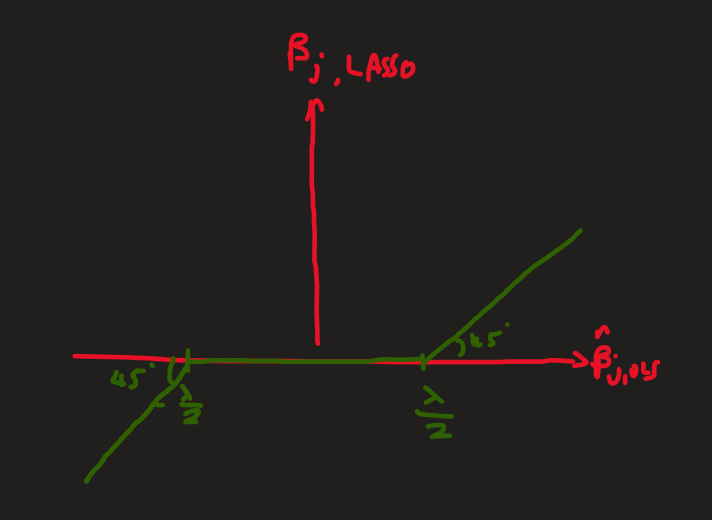
\includegraphics[width=0.7\textwidth]{soft thresholding lasso.png}
\end{center}
In contrast the ridge estimator in the orthonormal design case has form:
\[\hat{\beta}_{j,ridge}=(I+\lambda I)^{-1}X'Y=\frac{\hat{\beta}_{j,OLS}}{1+\lambda}\]
Thus it does not set any \(\hat{\beta}_{j,r}\) to zero. It just shrinks \(\hat{\beta}_{OLS}\).

\begin{note}
    As in practice we do not work inside the orthonormal design case, we need to standardise the regressors to make shrinkage apply fairly.
    Thus we demean all regressors to avoid shrinking the constant.
    And we divide all variables by their standard deviation to avoid shrinking variables with larger variance more, as this is unit variant.
\end{note}
\newpage
\section{Appendix}
\subsection{Proof Condition Number is Ratio of Eigenvalues}

\begin{theorem}
    For any positive definite symmetric matrix \(A\), the condition number \(C== ||A|| \, ||A^{-1}||\) is equal to the ratio of the largest eigenvalue to the smallest eigenvalue of \(A\).
    \[||A|| \, ||A^{-1}||=\frac{\lambda_{max}}{\lambda_{min}}\]
\end{theorem}

Recall that for any \underline{\smash{symmetric}} matrix \(A\), we have that \(A\) is diagonalisable (by spectral theorem). 
\\This means there exists an orthonormal basis of eigenvectors \((\vec{q_1},\, ...,\, \vec{q_n}) = Q\) that spans \(\mathbb{R}^n\), with corresponding eigenvalues \((\lambda_1,\, ...,\, \lambda_n), \, \text{where wlog} \, |\lambda_1|\geq|\lambda_2|\geq...\geq|\lambda_n|\).
\\Thus we can write any vector \(\vec{x}\in\mathbb{R}^n\) as a linear combination of these eigenvectors: \(\vec{x}=Q\vec{c}\)
\\Thus we can rewrite: \[||A||=\operatorname*{max}_{x\neq0}\frac{||Ax||}{||x||}=\operatorname*{max}_{x\neq0}\frac{||AQc||}{||Qc||}\]
\\\[=\operatorname*{max}_{x\neq0}\frac{||c_1\lambda_1q_1+...c_n\lambda_nq_n||}{||c_1q_1+...c_nq_n||}\]

Consider: \[\frac{||Ax||^2}{||x||^2}=\frac{(c_1\lambda_1q_1+...c_n\lambda_nq_n)'(c_1\lambda_1q_1+...c_n\lambda_nq_n)}{(c_1q_1+...c_nq_n)'(c_1q_1+...c_nq_n)}\]
\\
As eigenvectors orthonormal \(q_i'q_j=0\) for \(i\neq j\) and \(q_i'q_i=1\):
\[\therefore\,=\frac{c_1^2\lambda_1^2+...c_n^2\lambda_n^2}{c_1^2+...c_n^2}\leq\frac{c_1^2\lambda_1^2+...c_n^2\lambda_1^2}{c_1^2+...c_n^2}=|\lambda_1|^2\]
\[\implies \frac{||Ax||}{||x||}\leq|\lambda_1|\]
But we can achieve this bound at \(x=q_1\).
\vspace{5mm}
\begin{lemma}Thus:
\[||A||=\operatorname*{max}_{x\neq0}\frac{||Ax||}{||x||}=|\lambda_1|\]
\end{lemma}
For a \textit{positive definite} symmetric matrix we know that all \(\lambda_i>0\)
Thus \[||A||=\operatorname*{max}(\lambda_1,...,\lambda_n)\]

\begin{lemma}
    A matrix \(A\) has eigenvalue \(\lambda\) if and only if \(A^{-1}\) has eigenvalue \(\lambda^{-1}\).
\end{lemma}
\vspace{5mm}
\begin{proof}
Let \(v\) be an eigenvector of \(A\) with eigenvalue \(\lambda\). Then:
\[Av=\lambda v \implies A^{-1}Av=A^{-1}\lambda v \implies A^{-1}v = \frac{1}{\lambda}v\]
\end{proof}
\begin{lemma}
    \(A\) positive definite \(\implies A^{-1}\) (exists and is) positive definite.
\end{lemma}
\vspace{5mm}
\begin{proof}
    \(A\) positive definite implies \(A\) invertible, as only solution to Ax=0 is x=0 (thus full rank by rank nullity theorem). \\
    Consider for any \(x\in\mathbb{R}^n\) \[x'A^{-1}x\]
    Define \(x=Ay\) as for any \(x\) there must exist \(y\) where \(y=A^{-1}x\).
    Thus: \[x'A^{-1}x=(Ay)'A^{-1}(Ay)=y'A'y\]
    As \(y'A'y\) is a scalar, it is equal to its transpose. Thus:
    \[y'A'y=(y'A'y)'=y'Ay>0 \quad \text{as A positive definite}\]
    Thus \(A^{-1}\) is positive definite.
\end{proof}

Thus, as \(A^{-1}\) positive definite:
\[||A^{-1}||=\operatorname*{max}(\lambda_1^{-1},...,\lambda_n^{-1})\]
As \(\lambda_i>0\) for all \(i\),
\[||A^{-1}||=\frac{1}{\lambda_{min}}\]
Thus:\[C=||A|| \, ||A^{-1}||=\frac{\lambda_{max}}{\lambda_{min}}\]

\begin{note}
We can apply this to the regression case by considering \(A=X'X\) so long as \(X'X\) is positive definite. We prove that \(X'X\) is positive definite if \(X\) is full rank and \(n>k\):
This is because for any vector \(\alpha\neq0\) we have:
\[\alpha'X'X\alpha=(X\alpha)'X\alpha=||X\alpha||^2\geq0\]

To show inequality is strict, we must show that the null space of \(X'X\) is trivial.
We are given \(null(X)\) is empty as \(X\) is full rank by rank nullity theorem, thus we simply must show \(null(X'X) = null(X)\). (only true for real matrices)
\\ \\
\(\underline{null(X)\subseteq null(X'X)}\):
\[\text{Let vector} \, v\in null(X), \text{then} \, Xv=0\]
\[\implies X'Xv=X'0=0\]
\[\implies v\in null(X'X)\]

\(\underline{null(X'X)\subseteq null(X)}\):
\[\text{Let vector} \, v\in null(X'X), \text{then} \, X'Xv=0\]
\[\implies v'X'Xv=0\]
\[\implies ||Xv||^2=0\]
\[\implies Xv=0 \quad \text{provided X is real valued}\]
\[\implies v\in null(X)\]

Thus \(null(X'X)=null(X)=0\) and \(X'X\) is positive definite.
\end{note}

\subsection{Proof Condition Number Bounds Solution Sensitivity}

\begin{theorem}
    For a set of simulateneous equations \(Ax=b\) the condition number of \(A\) sets a bound of the sensitivity of the relative (i.e. invariant to units) solution error (in \(x\)) induced by errors in the problem vector (\(b\)). \(\frac{||\Delta x||}{||x||} \leq C \frac{||\Delta b||}{||b||}\)
\end{theorem}

\vspace{5mm}

\begin{proof}

Recall the submultiplicity property of the norm:
\[||Ax||\leq||A||\,||x||, ||AB||\leq||A||\,||B||\]

Suppose there exists a problem error in \(b\) such that \(\tilde{b}=b+\Delta b\).
\\ Then the solution to the new problem is \(\tilde{x}=A^{-1}\tilde{b}\). We seek a bound on the unit invariant relative error in the solution:

Consider:
\[A(x+\Delta x)=b+\Delta b\]
\[Ax=b\implies A\Delta x=\Delta b \implies \Delta x=A^{-1} \Delta b\]
\[\implies ||\Delta x||\leq||A^{-1}||\,||\Delta b||\]
But:
\[Ax=b\]
\[\implies ||b||\leq||A||\,||x||\]
Now multiplying inequalities:
\[||\Delta x||\,||b||\leq||A^{-1}||\,||\Delta b||\,||A||\,||x||\]
\[\implies \frac{||\Delta x||}{||x||}\leq||A^{-1}||\,||A||\frac{||\Delta b||}{||b||}\]
\end{proof}

\subsection{Proof Ridge Regression Reduces Condition Number}
\vspace{5mm}
\begin{theorem}
    Let \(A\) be a positive definite symmetric matrix with condition number:
    \[C=||A||\,||A^{-1}||=\frac{\lambda_{max}}{\lambda_{min}}\]
    Then the condition number of \((A+\mu I)\) is:
    \[\frac{\lambda_{max}+\mu}{\lambda_{min}+\mu}<\frac{\lambda_{max}}{\lambda_{min}}\]
\end{theorem}
\vspace{5mm}
\begin{proof}
    Let Q be an orthonormal basis of eigenvectors of A, with corresponding eigenvalues \(\lambda_1,...,\lambda_n\). Then:
    \[(A+\mu I)Q=AQ + \mu IQ=Q\Lambda + Q\mu I=Q(\Lambda + \mu I)\]
    Thus we can diagonalise (A+\(\mu\)I) with eigenvalues \(\lambda_1+\mu,...,\lambda_n+\mu\) as follows.
    \[(A+\mu I)=Q(\tilde{\Lambda} + \mu I)Q'\]
    Where \(Q\) is the same orthonormal basis, and all eigenvalues are simply augmented by \(\mu\).
    \\Thus: \[\frac{\tilde{\lambda}_{max}}{\tilde{\lambda}_{min}}=\frac{\lambda_{max} + \mu}{\lambda_{min} + \mu}\]
\end{proof}

\begin{note}
    \[Q'=Q^{-1}\]
    \[\because Q'Q=QQ'=I\]
\end{note}

\end{document}